\subsection{Front-end Clients}
\subsubsection{Single Codebase}
In the design document, we'd envisioned two different codebases for the different edge (mobile) and management (desktop) clients. During development, however, it has become obvious that a single codebase with client side routing and bundle separation using tree shaking was more suitable for our application. We are bundling both applications in a single router, and there is no clear separation between each client. During development, special care was given to reduce cross dependencies between both parts to a minimum in order to reduce the bundle size for edge devices.

\subsubsection{/lib folder}
Originally, there were only two auxiliary classes in the whole client (MobileAPI and DesktopAPI), while everything else was a React component. During development, we made use of custom react hooks (/lib/hooks) to refactor common stateful logic into reusable parts. Apart from hooks, sensor data collection needed it's own abstraction over the clunky Web API implementation, which we've placed in /lib/sensors.

\subsubsection{API endpoints}
In order to accomodate changes in the backend, both the Mobile- and DesktopAPI have undergone major changes in the interfaces they implement.

\subsubsection{Component Library}
In the design document, we'd specified Material-UI as the component library that we were going to use. During development we've found it too clunky, heavy and hard to develop with and replaced it with the Evergreen Component Library from segment.io. This component library also comes with it's own opinionated 'CSS-in-JS' styling library, through which we were able to style the application with a rapid pace.

\subsubsection{ModelOptions Component}
This component faced the most changes during implementation. We'd decided to distribute some model creation options to the sensor-components themselves instead of using the same set of parameters for each component. This had it's implications on the client and it had to be updated accordingly.

\begin{figure}[!htbp]
    \centering
    \fbox{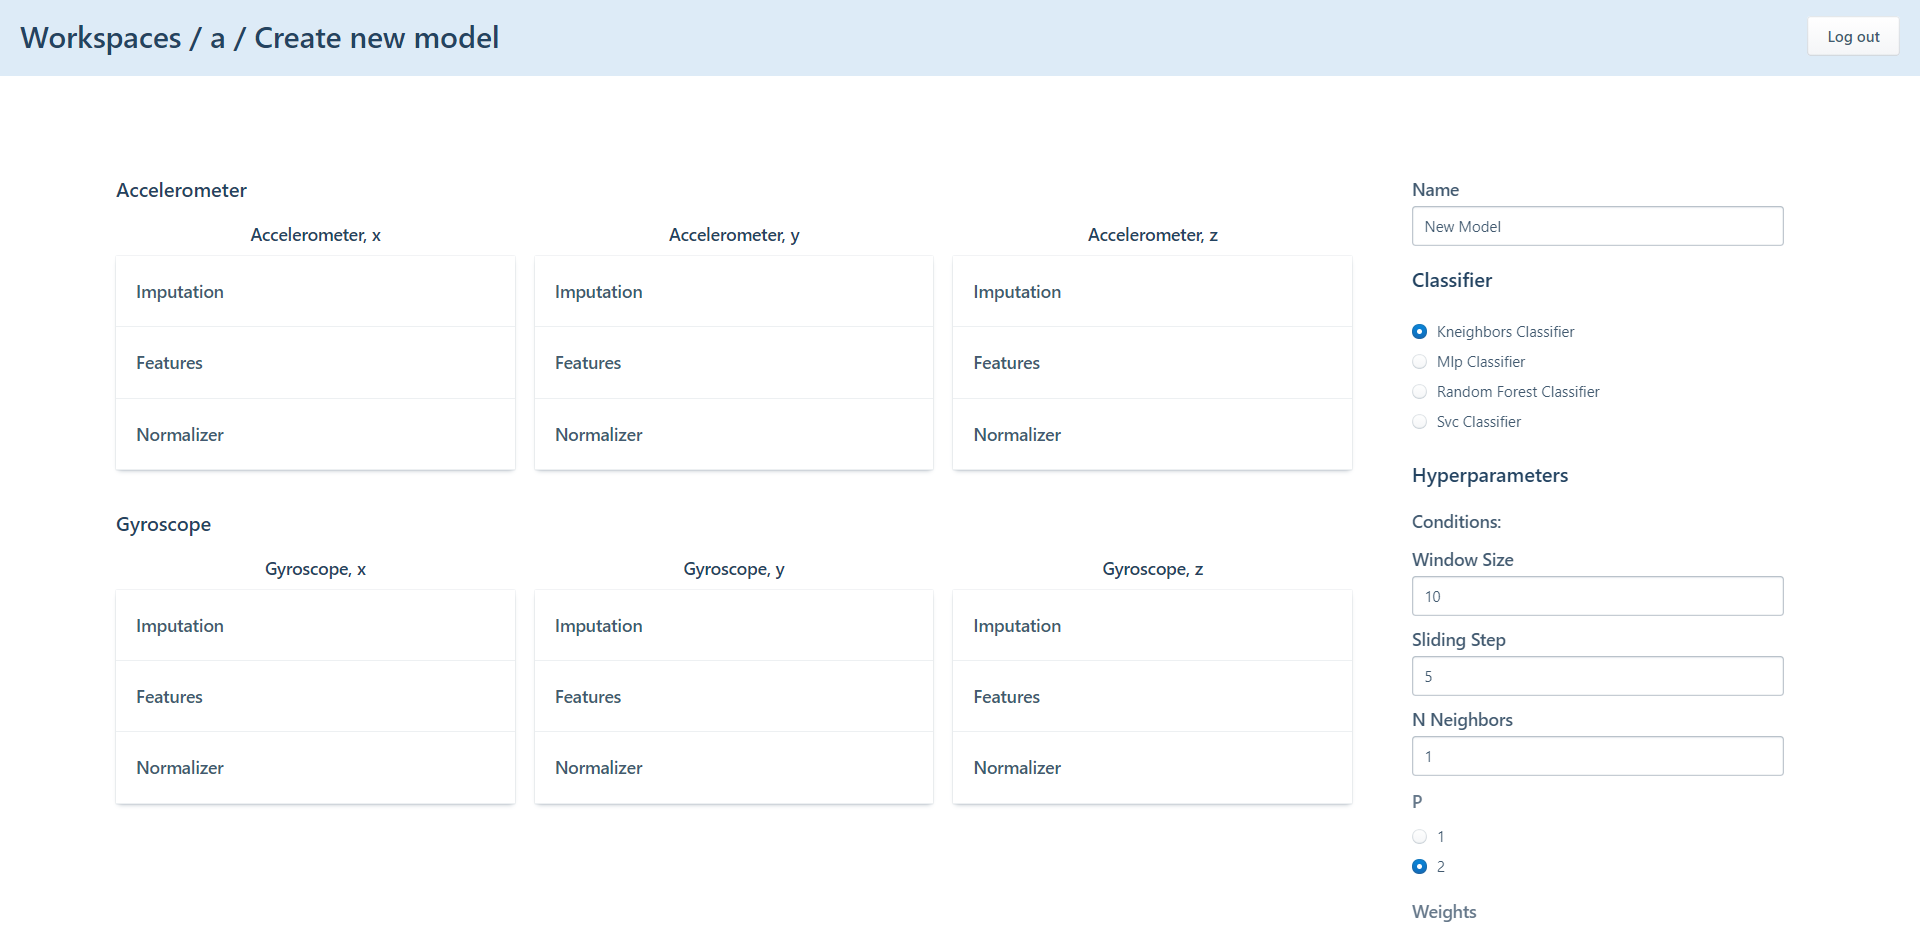
\includegraphics[width=\textwidth]{images/v-modelpng.png}}
    \caption{New ModelOptions}
\end{figure}

% \begin{figure}[!htbp]
%     \centering
%     \fbox{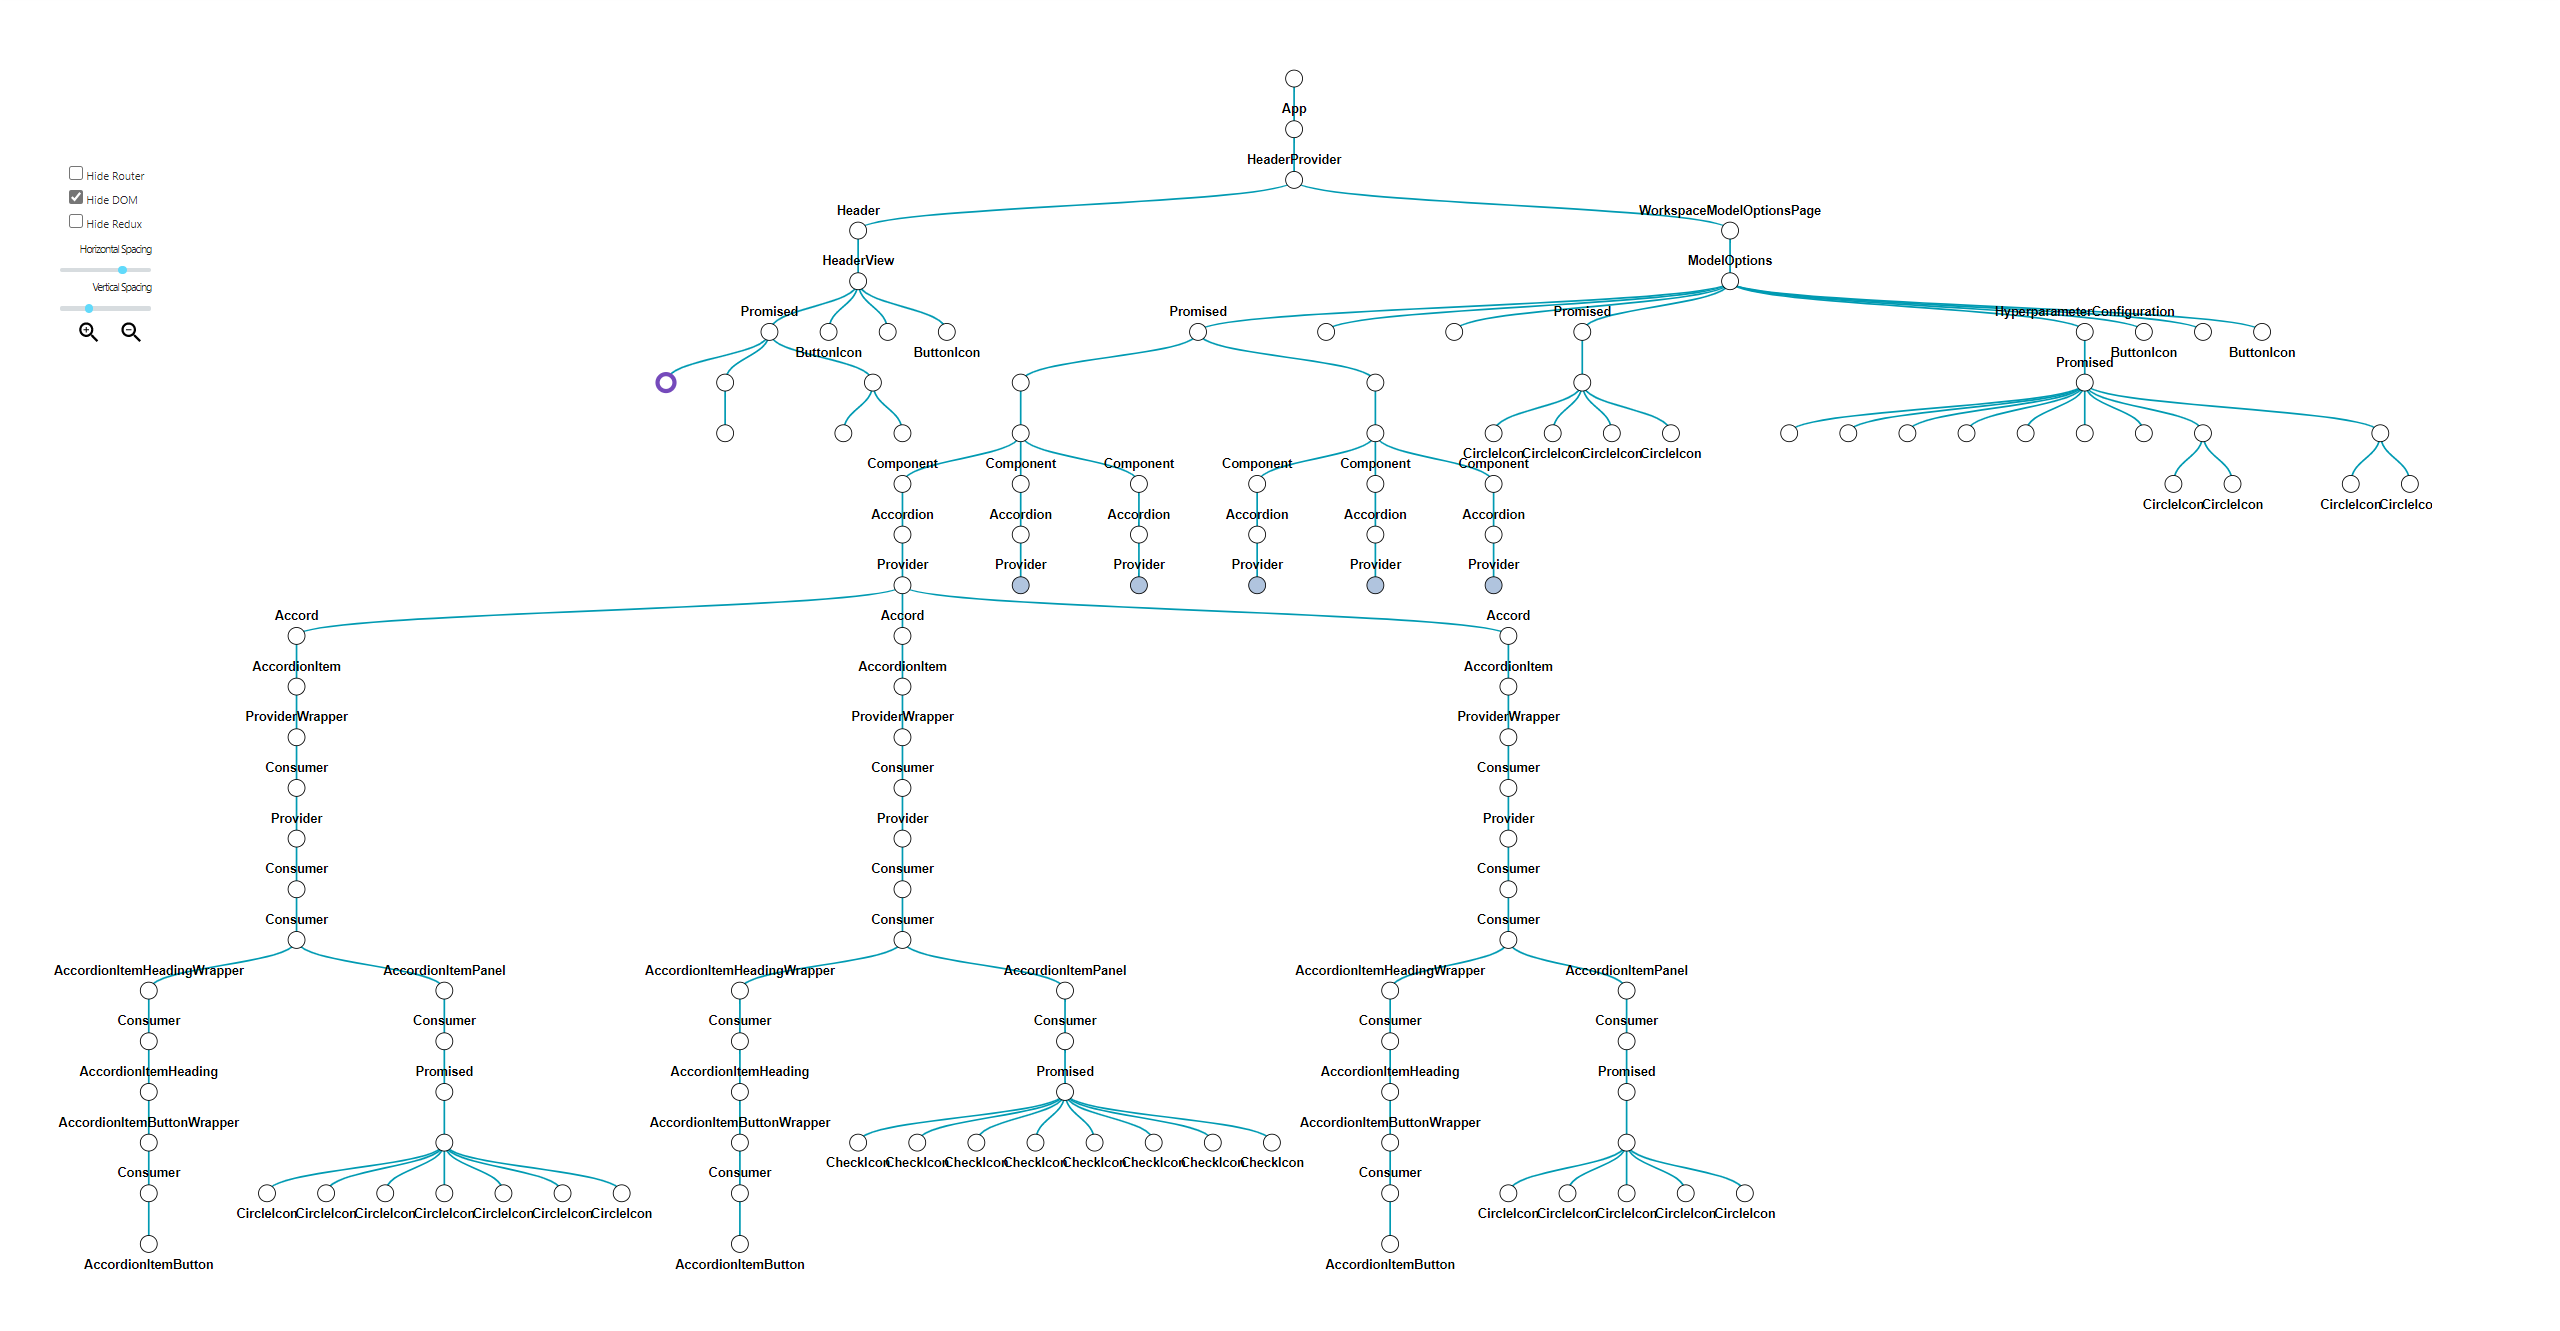
\includegraphics[height=1.2\textheight]{images/ch-model.png}}
%     \caption{New ModelOptions Component Graph}
% \end{figure}

\subsubsection{Class/Component Diagram}
For the updated component diagram, please see the `Client Diagram.png` in the same folder as this document. It is also attached at the end of this document.
\begin{figure}[!htbp]
    \centering
    \fbox{\includegraphics[height=0.15\textheight]{images/src_diagram.png}}
    \caption{Overview of the updated diagram. Can be found in the appendix in full resolution.}
\end{figure}